% !TeX root = ../../../book.tex
\section{数学陈述}

我们首先要做的是讨论哪些类型的句子可以合理地视为需要证明或证伪的数学真理。完成这一步其实是相当困难的!许多作者倾向于忽略这个主题或仅提供一个简单的定义,而忽略了数学语言和逻辑的许多微妙之处。我们也感到束手无策,因为本书/课程提供的时间和空间不足以正确研究抽象逻辑理论领域。我们鼓励你阅读一些包含相关信息的书籍或网站。就目前的情况而言,我们必须隐藏许多细节。不过,换句话说,数学研究有一个非常深入、丰富和富有成果的领域,这正是我们将在本章以更具启发性的方式讨论的内容。

请记住,我们提到过我们必须假设实数 $\mathbb{R}$ 存在及其常规算术属性。同样,我们会假设数理逻辑的许多结果和概念,这些你通常甚至都没有意识到(直到我们给你指出)。这些细节可以在你以后的数学生涯中更深入地研究。

% !TeX root = ../../../book.tex
\subsection{定义}

现在,让我们讨论一下\textbf{数学陈述}的含义。我们希望这个术语能够概括我们可以证明或证伪的``事物''类型。

数学在科学中是独一无二的,因为该领域的结果经过严格\textbf{证明},而不是先做出假设然后通过实验室实验或现实世界观察来``证实''。在数学中,我们假设一组常见的\textbf{公理},然后遵循严格的逻辑推理,从这些公理(以及迄今为止我们已经证明的其他真理)中推导出真理。如果我们遇到虚假信息,我们就必须证明或揭示它确实为假。

基于上述想法,我们来看几个\textbf{数学陈述}或\textbf{命题}可能是什么的例子。(我们甚至已经证明了其中一些!)例如,这句话:
\begin{center}
    \textcolor{olivegreen}{对于任意实数 $x, y \in \mathbb{R}$,不等式 $2xy \le x^2 + y^2$ 成立。}
\end{center}
是一个有效的数学陈述。事实上,它是真的,我们将在稍后的 \ref{sec:section4.9.2} 节中证明这一点。(它有时被称为 AGM 不等式,是\emph{算术几何平均不等式(Arithmetic-Geometric Mean Inequality)}的缩写。)这里需要指出,``成立''一词在数学中经常用于表示``为真''或``是一个真实的陈述''。

下面是另一个数学陈述的例子:
\begin{center}
    \textcolor{olivegreen}{对于任意集合 $S, T, U$,如果 $S \cap T \subseteq U$ 则 $S \subseteq U$ 或 $T \subseteq U$。}
\end{center}

然而,上面这种说法是错误的,如以下反例所示:
\begin{center}
    \textcolor{blue}{设 $S = \{1, 2, 3\}$, $T = \{2, 3, 4\}$, $U = \{2, 3, 5\}$。\\ 很明显 $S \cap T = \{2, 3\} \subseteq U$ 但 $S \nsubseteq U$ 且 $T \nsubseteq U$。}
\end{center}
为什么这个例子证伪了上面的说法?你弄明白了吗?你能解释一下吗?我们将在本章后面更详细地讨论这一点,但我们希望现在我们都认识到这个例子确实实现了这一点。

我们也都认同像这样的句子
\begin{center}
    \textcolor{red}{为什么我们早上 9:00 还要上课?!}
\end{center}
绝对\textcolor{red}{\emph{不是}}数学陈述。这是一个完全有效的句子,但从数学上来讲它没有意义:我们无法\emph{证明}或\emph{证伪}它。

同理,这句话
\begin{center}
    \textcolor{red}{$x^2 - 1 = 0$}
\end{center}
尽管完全由数学符号组成,但它也\textcolor{red}{\emph{不是}}数学陈述。问题是我们无法纯粹从公理和逻辑推论来验证它为真还是为假。该陈述\emph{取决于} $x$,无论该值是什么(即 $x$ 是一个\textbf{变量}),并且在不对其施加额外假设的情况下,我们无法断言该句子为真还是为假。这种类型的句子稍后将被称为\textbf{变量命题}:其真实性取决于句子中的变量。

所有这些观察结果和示例/伪例引出了以下定义:

\begin{definition}
    \dotuline{数学陈述}(或\dotuline{命题}或\dotuline{逻辑陈述})是语法正确的句子(或句子串),由单词/标点符号和数学符号组成,并具有唯一一个真值(真或假)。
\end{definition}


% !TeX root = ../../../book.tex
\subsection{示例和伪例}

``语法正确''是指句子中的单词和符号被正确组合且具有明确含义。这排除了无意义的符号或单词组合,例如:
\begin{center}
    \textcolor{red}{$1+ = 2$, $\text{Fisher}^2 = 1$, $\big\{\{\varnothing\}\big\} - 7 > 5\pi$, $\text{You am smart}$}
\end{center}
以上第三个例子并非数学陈述,因为 $\big\{\{\varnothing\}\big\}$ 不是数字,无法解释如何从该集合中``减去 $7$''。

而``\emph{唯一}真值''要求陈述要么为\verb|真|要么为\verb|假|,不能同时成立,也不能非真非假。这排除了``\textcolor{red}{$x^2 - 1 = 0$}''这类陈述——若未声明 $x$ 的取值,则无法判定其真值。

\subsubsection*{真值未知}

定义中的有趣之处在于:即使能确定真值唯一,我们仍可能不知其具体结果。例如:
\begin{center}
    \textcolor{olivegreen}{任何大于或等于 $4$ 的偶自然数均可表示为两个质数之和。}
\end{center}

此命题是真是假?若能证明或证伪,数学界将为之振奋!该命题称为\href{https://baike.baidu.com/item/哥德巴赫猜想/72364}{哥德巴赫猜想}\footnote{术语说明:\textbf{猜想}指被认为成立但尚未被证明或证伪的命题。},是数学中著名的未解难题(我们相信只是暂时的!)。尽管目前无人知晓其真伪,可以肯定的是,\emph{仅有一个}真值适用:该命题不可能既\verb|真|又\verb|假|,也不可能存在中间状态。要么所有不小于 $4$ 的偶自然数都具有此性质,要么存在反例。即使尚未知晓正确答案,这种``非此即彼''的特性仍然成立。因此该命题完全满足\emph{数学陈述}的定义。

\subsubsection*{悖论语句}

使陈述没有真值的一种方法是构造\textbf{悖论}。考虑以下陈述:
\begin{center}
    \textcolor{red}{这句话是假的。}
\end{center}
这显得十分怪异,因为该语句直接断言了自身的真值。现在分析其可能的真值:
\begin{itemize}
    \item 假设这句话为\verb|真|。那么,根据其内容,它实际上为\verb|假|。
    \item 假设这句话为\verb|假|。同理,根据其内容,它实际上为\verb|真|。
\end{itemize}
这种矛盾无法调和!这句话某种程度上同时具有\verb|真|与\verb|假|的双重属性,或处于某种非真非假的状态。由于数学体系需要避免此类异常现象,我们的定义将明确排除这类语句。

(\emph{思考题}:若允许此类语句作为合法数学陈述,会产生什么后果?若放弃``每句话必为\verb|真|或为\verb|假|''的基本原则,数学体系是否仍能自洽?这会引发矛盾,还是创造出一个全新的数学宇宙?)

通常,这种\textbf{自指}语句(即指向自身的陈述)极易引发悖论,这正是我们需要禁止的。

\begin{multicols}{2}
    该悖论的变体可以通过右侧这幅卡通漫画说明:当皮诺曹说``我的鼻子要变长''时会发生什么?若此言为真,则鼻子会伸长——但皮诺曹的鼻子仅在说谎时才会变长。若此言为假,则鼻子会伸长(符合说谎特征),而这反而验证了陈述的真实性!如此形成无法解开的逻辑循环。

    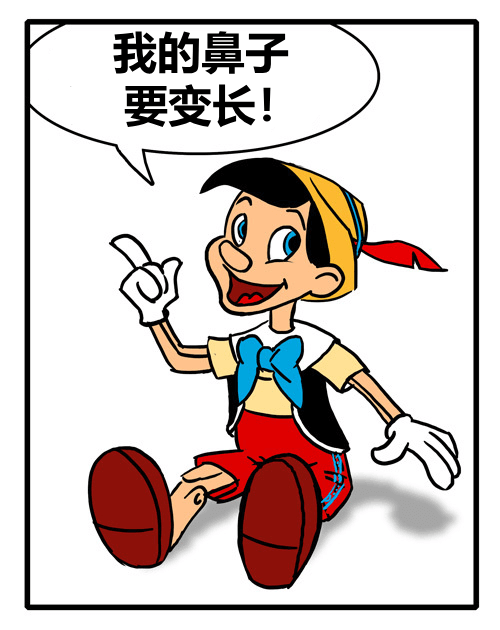
\includegraphics[scale=0.3]{figure/pinocchio.png}
\end{multicols}

更复杂的案例是\emph{奎因悖论 (Quine's Paradox)}:
\begin{center}
    \textcolor{red}{``Yields falsehood when preceded by its quotation'' \\yields falsehood when preceded by its quotation.}
\end{center}
此悖论留待读者自行探索。此类自相矛盾的陈述具有本质上的病态特征,因此我们的定义将直接排除它们。


% !TeX root = ../../../book.tex
\subsection{变量命题}

另一类非数学陈述涉及\textbf{未量化变量}。例如:
\begin{center}
    \textcolor{red}{``$x^2 - 1 = 0$''}
\end{center}

该语句在语法上是正确的,我们也能理解它,但其真值无法确定:当 $x = 1$ 时为\verb|真|,当 $x = 8$ 时为\verb|假|;若 $x = \mathbb{N}$ 或 $x = \text{Fisher}$,则该语句无意义。因此这类语句也应被排除。鉴于其广泛用途,我们称之为\textbf{变量命题},因为其主张\emph{依赖于}特定变量。

对于上述语句,可定义变量命题 $P(x)$ 表示 ``$x^2 - 1 = 0$'',通常表述为:
\begin{center}
    \textcolor{olivegreen}{令 $P(x)$ 表示命题``$x^2 - 1 = 0$''。}
\end{center}
惯例上用大写字母表示变量命题,小写字母表示所含变量(非强制要求)。

定义变量命题后,可通过为变量 $x$ \emph{赋值}生成有效的数学陈述:如 $P(1)$ 为真,$P(0)$ 为假。亦可对 $P(x)$ 进行\textbf{量化},例如,下面的语句是一个为\verb|真|的数学陈述:
\begin{center}
    存在 $x \in \mathbb{R}$ 使得命题 $P(x)$ 为\verb|真|。
\end{center}
而下面的语句是一个为\verb|假|的数学陈述:
\begin{center}
    对于每个 $x \in \mathbb{R}$,命题 $P(x)$ 均为\verb|真|。
\end{center}
请思考这些陈述的真值依据及其数学陈述属性,并考虑如何证明。

\subsubsection*{定义变量命题}

定义变量命题需遵循特定格式:
\begin{enumerate}[label=(\arabic*)]
    \item 为命题分配字母名称(如 $P$);
    \item 标明其依赖变量(如 $x$ 或 $y$);
    \item 为实际命题添加引号;
    \item 避免引入命题上下文之外的字母。
\end{enumerate}
此格式经过严谨设计以确保精确性:明确界定命题中各字母的含义,清晰区分命题内容与外部要素。

例如,以下是变量命题的\textcolor{red}{\textbf{不当}}``定义''示例。我们将分析其问题所在,并提出修改建议。
\begin{itemize}
    \item \textcolor{red}{令 $Q(y)$ 为命题``$x < 0$''。}\\
        \textbf{问题}:$x$ 未定义,且 $y$ 未在命题中出现,变量使用混乱。\\
        \textbf{修改为}:
        \begin{center}
            \textcolor{olivegreen}{令 $Q(x)$ 为命题``$x<0$''。}
        \end{center}
        此时括号内变量与命题变量一致,是良好的定义。
    \item \textcolor{red}{对于每个 $x \in \mathbb{R}$,令 $P(x)$ 为命题 $x^2 \ge 0$。}\\
        \textbf{问题}:量词``对于每个''可能被误解为命题组成部分,导致语义歧义。\\
        若将其解释为针对每个 $x \in \mathbb{R}$,逐一定义 $P(x)$ 为``$x^2 \ge 0$'',这或许成立;\\
        但若将其理解为 $P(x)$ 定义为``对于每个 $x \in \mathbb{R}$, $x^2 \ge 0$'',则不构成正确定义的命题——命题内的变量不应被重复量化。\\
        该命题的原始写法有两种可能的解释,而且它们非常不同。因此,这是一个不当的定义。\\
        \textbf{修改为}:
        \begin{center}
            \textcolor{olivegreen}{对于每一个 $x \in \mathbb{R}$,定义 $P(x)$ 为命题``$x^2 \ge 0$''。}
        \end{center}
        明确量词作用范围可消除歧义。虽然变量定义域并非必需,但明确说明并无不妥。
    \item \textcolor{red}{令 $T(x, y)$ = ``$x^2 - 7 = y$''。}\\
        \textbf{问题}:这里的``$=$''是什么意思?当我们希望比较两个数字并说它们的值相等(或比较两个集合并说它们的元素相同)时,该符号才有意义。对象 $T(x, y)$ 是一个数学陈述,要么为\verb|真|,要么为\verb|假|。因此,它没有数值可以与其他任何东西进行比较。\\
        同理,给定 $x$ 和 $y$ 的值,语句 ``$x^2 - 7 = y$'' 要么为\verb|真|,要么为\verb|假|,因此说该方程``等于''其他值是没有意义的。它具有真值,而非数值。\\
        \textbf{修改为}:
        \begin{center}
            \textcolor{olivegreen}{令 $T(x, y)$ 为``$x^2 - 7 = y$''。}
        \end{center}
        就变成有效的变量命题。
\end{itemize}

我们无意过多列举错误示例,但教学经验表明,这些是学生定义命题时的常见疏漏(无论是否意识到其错误性),故特此说明。

最后需要明确一点:定义命题时不必预先说明变量从何而来。例如定义
关于变量命题最后有一点说明。定义命题时不必说明变量从何而来。可以稍后在调用命题时或者使用变量的特定值时填写。也就是说,我们可以定义
\begin{center}
    令 $T(x, y)$ 为``$x^2 - 7 = y$''。
\end{center}
无需指定 $x,y$ 到底是自然数、整数、复数还是其他类型数字。后续可验证 $T(3, 2)$ 为\verb|真|,$T(\pi, -1)$ 为\verb|假|,$T(\varnothing, \mathbb{N})$ 无意义。但在定义 $T(x,y)$ 时,我们无需预设这些具体解释。


% !TeX root = ../../../book.tex
\subsection{词序至关重要!}\label{sec:section4.2.4}

我们将在下一节中详细讨论\textbf{量化}变量的概念。现在,我们想考虑一个更加引人注目的数学陈述示例,它说明了语句中词序的重要性。分析如下语句的结构也将是下一节的主要目标。
\begin{center}
    存在一个实数 $y$,使得对于每个实数 $x$, $y = x^3$。
\end{center}
这个句话说了什么?它说的是无论 $x \in \mathbb{R}$ 是什么,我们都可以找到一个数字 $y \in \mathbb{R}$ 使得 $y = x^3$ 为\verb|真|。这是荒唐的!怎么可能有一个数字是所有数字的立方呢?这句话确实是一个数学陈述,但它绝对为\verb|假|。但下面的说法又如何呢?
\begin{center}
    对于每个实数 $x$,存在一个实数 $y$,使得 $y = x^3$。
\end{center}
上面这句话为\verb|真|!你看出两个句子之间的区别了吗?它们包含完全相同的单词和符号,但顺序不同。前一句断言存在某个数字是每个实数的立方(此为\verb|假|),而后一句断言每个实数都有一个立方根,此为\verb|真|。这个例子强调了词序的重要性。


% !TeX root = ../../../book.tex
\subsection{习题}

\subsubsection*{温故知新}

以口头或书面的形式简要回答以下问题。这些问题全都基于你刚刚阅读的内容,如果忘记了具体定义、概念或示例,可以回顾相关内容。确保在继续学习之前能够自信地作答这些问题,这将有助于你的理解和记忆!

\begin{enumerate}[label=(\arabic*)]
    \item 数学陈述的关键定义属性是什么?
    \item 数学陈述与变量命题有何区别?
    \item 为什么哥德巴赫猜想是一个数学陈述?
    \item 以下定义变量命题的尝试存在什么问题?
        \begin{center}
            \textcolor{red}{令 $Q(x, y, z)$ 为 $7x - 5y + z$}
        \end{center}
\end{enumerate}

\subsubsection*{小试牛刀}

尝试解答以下问题。这些题目需动笔书写或口头阐述答案,旨在帮助你熟练运用新概念、定义及符号。题目难度适中,确保掌握它们将大有裨益!

\begin{enumerate}[label=(\arabic*)]
    \item 对于以下每个语句,判断其是否为数学陈述。若是,请判断其\verb|真|\verb|假|;若不是,请解释原因。
        \begin{enumerate}[label=(\alph*)]
            \item $142857 \cdot 5 = 714285$
            \item 对于每个 $n \in \mathbb{N}$, $\displaystyle{\sum_{k \in [n]}k=\frac{n(n+1)}{2}}$。
            \item 对于任意集合 $A$ 和 $B$,若 $A \subseteq B$,则 $B \subseteq A$。
            \item 对于任意集合 $A$ 和 $B$,若 $A \subseteq B$,则 $\mathcal{P}(A) \subseteq \mathcal{P}(B)$。
            \item 数学就是酷。
            \item $1 + 2 = 0$
            \item 对于任意 $x, y \in \mathbb{Z}$,若 $x \cdot y$ 为偶数,则 $x$ 和 $y$ 均为偶数。
            \item 对于任何 $x, y \in \mathbb{Z}$,若 $x$ 和 $y$ 均为偶数,则 $x \cdot y$ 也为偶数。
            \item $1+ = 2$
            \item $-5 + \mathbb{Z} \ge \pi$
            \item $x = 7$
            \item 这句话不正确。
        \end{enumerate}
    \item 回顾前三章,找出数学陈述的一些例子和伪例。\\
    你能发现变量命题吗?它们是否按本节指定的方式编写?能否修正其中不当的书写?
    \item 写出一个变量命题的正确定义,要求当两个输入值之和为非负时,该命题为真。\\
    然后,找出命题为\verb|真|和为\verb|假|时的两个实例。
    \item 令 $S$ 为集合 $\{1, 2, 3, 6, 8, 10\}$。
        \begin{enumerate}[label=(\alph*)]
            \item 编写一个变量命题的正确定义,接受两个变量输入,并判断其差的绝对值是否为 $S$ 的元素。然后,分别找出命题为\verb|真|和为\verb|假|时的两个实例。
            \item 编写一个变量命题的正确定义,接受两个集合输入,并判断其交集是否为 $S$ 的子集。然后,分别找出命题为\verb|真|和为\verb|假|时的两个实例。
        \end{enumerate}
        (注意:对任意集合 $X$ 和任意对象 $x$,必有 $x \in X$ 或 $x \notin X$。)
    \item 构想另一个数学命题,其原始陈述为\verb|真|,但交换部分词语顺序后变为\verb|假|。(参考最后一小节的示例以获取灵感。)
    \item 对于以下变量命题定义,判断其是否合理。注意:此处并非判断其\verb|真|\verb|假|,而是评估其表述是否规范。\\
    若存在错误,请解释原因并修正该定义。
    \begin{enumerate}[label=(\alph*)]
        \item 令 $P(x)$ 为``$x > 1$''。
        \item 令 $Q(x)$ 为命题``$x^2 - 1 > 0$''。
        \item 对于每个 $a,b \in \mathbb{R}$,令 $R(a, b)$ 为``$a^3 = b$''。
        \item 令 $P(x)$ 为 $x > 1$。
        \item 令 $T(z) = $ 为``$z$ 为质数''。
        \item 令 $Q(x)$ 为命题``$x^2 - 1 > 0$'',其中 $x \in \mathbb{R}$。
        \item 对于每个 $x \in \mathbb{R}$,令 $Q(x)$ 为``$x^2 - 1 > 0$''。
        \item 令 $S(a)$ 为 ``$b^2 > 4$''。
        \item 令 $Q(x)$ 为 $x^2 - 1 > 0$ 其中 $x \in \mathbb{R}$。
    \end{enumerate}
\end{enumerate}